\section*{{Abstract:}}


	Lower residents are often reliant on public transit for daily travel. They have also historically concentrated in centrally located neighbourhoods with relatively higher levels of transit accessibility. However, during the late 20th and early 21st century, many urban regions have undergone trends of inner-city gentrification and suburbanization of poverty, raising concerns that low-income residents are disproportionately moving away from relied upon transit service. In this paper, we investigate what occurs when low-income residents change dwellings within a region: do they experience a reduction in their levels of transit accessibility, how does this compare to higher-income movers, and how has this changed over time? We examine this by linking historical transit accessibility measures to annual individual-level panel data representing 20\% of tax filers in Toronto, Canada from 1988 to 2018. We then analyze changes in transit accessibility for intra-urban movers via descriptive statistics and regression models to answer whether there are significant differences in individual changes in transit accessibility by low-income status. We find that low-income residents do, on average, experience reductions in their levels of transit accessibility when moving within the region, but they do not undergo as great of a reduction in transit accessibility as higher-income movers. However, the gap in experienced changes in transit accessibility between high- and low-income movers is converging over time.


\section*{{Keywords:}}

transit accessibility, residential mobility, income, displacement, exclusion



\section{Introduction}

Public transit is immensely important among lower-income urban residents for daily travel \cite{sanchez_transit_2004,giuliano_low_2005,kramer_unaffordable_2018,barri_can_2021}. In most cities, transit accessibility is greater near the centre than in more peripheral neighbourhoods. While lower-income residents tend to live in areas of greater transit accessibility on average \cite{deboosere_evaluating_2018,allen_sizing_2019}, some North American cities have undergone trends of inner-city gentrification and suburbanization of poverty over the past several decades \cite{kneebone_suburbanization_2010,ehrenhalt_great_2012,ades_are_2012, grant_changing_2020}. This means that in some places, lower-income households are increasingly living in areas with relatively lower levels of transit accessibility and thus have greater barriers to daily travel and are facing increased risks of transport-related social exclusion \cite{allen_suburbanization_2021,liu_suburbanization_2021}. 

There are also growing concerns that some transit rich neighbourhoods are becoming unaffordable and are resulting in the residential displacement and exclusion of low-income residents; but quantitative studies have mixed or inconclusive results about whether low-income residents move disproportionately out of gentrifying neighbourhoods or whether newly built transit lines directly leads to the displacement of low-income residents \cite{rayle_investigating_2015, zuk_gentrification_2018,padeiro_transit-oriented_2019,delmelle_transit-induced_2021}. However, existing research that studies income inequalities of residential mobility in relation to public transit focuses on the outcomes of specific transit routes, which serve only a fraction of the population in a region, rather than comprehensively examining changes across an entire region. As such, there is needed research to assess whether there are social inequalities at a regional level pertaining to whether lower-income residents are unequally reducing their levels of transit accessibility when they move. 

The objective of our paper is thus to answer the following: do low-income residents, on average, experience a reduction of their level of transit accessibility when they move within a region? If so, to what extent? And if so, do low-income movers witness a greater reduction in transit accessibility than higher-income movers? Specifically, we examine differences in transit accessibility resulting from intra-urban moves using an administrative dataset representing 20\% of tax-filers across an entire region (Toronto) over a 30-year period (1988 to 2018). Findings of this study are important for understanding whether there is evidence of a disproportionate number of low-income residents moving away from much relied upon public transit service, and if so, how this has changed over time. Furthermore, findings about differences in individual residential mobility patterns by income and relative to transit accessibility can offer further explanations about how contemporary trends of urban socio-spatial restructuring, such as inner-city gentrification and suburbanization of poverty, unfold within a region over time. While our empirical analysis is focused on a single region, the types of data and methods described in our paper could be applied to other regions.







\section{Background}

Many North American cities, throughout much their histories, have been characterized with income profiles of increasing wealth from the inner-city (typically where there is adequate transit service) outwards towards the suburbs (where cars are often a necessity for daily travel). Early 20th century urban sociologists described residents as moving up the social hierarchy by moving out away from the city via processes of succession and filtering, while more central neighbourhoods were places for in-migration and the working class \cite{burgess_growth_1925}. Monocentric urban conceptualizations have also been used in urban land-use theory \cite{alonso_location_1964} to explain why lower-income residents have concentrated centrally; that while households and firms make trade-offs between commuting/travel costs and housing size, the elasticity for living space for households is greater than that for travel costs, leading to central-peripheral income gradients \cite{becker_theory_1965,glaeser_why_2008}. 

The historical concentration of low-income residents in central parts of cities rather than the suburbs has also been theorized in terms of both preferences and constraints. Concentration of poverty within central areas is associated with living in a neighbourhood in which the population is overwhelmingly socially disadvantaged (e.g. crime, urban decay, pollution) as well as inaccessibility to sufficient social and community resources such as education and employment \cite{wilson_truly_2012, lucas_transport_2012,sampson_great_2012}. Such conditions can also act as push-factors persuading out-moving of residents who can afford to do so \cite{jones_neighbourhood_2021}. Land-use and transport planning can also be factors in the residential location of low-income residents in more centrally located neighbourhoods, specifically clustering in areas with greater transit accessibility. For instance, usually under sustainability objectives, regions often try to plan higher density housing (e.g. apartments) to be co-located near major transit nodes and corridors (often termed as transit-oriented development). Overall, apartments tend to have better transit connections and are also more likely to be home to low-income residents than lower-density residential dwellings. Lower-income residents also tend to have greater preferences to live near transit because of the high costs of private vehicles \cite{glaeser_why_2008}. For similar reasons, immigrants with lower incomes, on average, often tend to settle in central areas rather than in the suburbs. Immigrants also often face delays in acquiring drivers licenses, further causing reliance on and preferences for public transit \cite{blumenberg_getting_2010,blumenberg_planning_2010,lo_relationship_2011}. 

Individual decisions to move are often conceptualized as a more complex combination of household preferences at different stages-of-life as well as built environment factors, both in terms of push factors away from a neighbourhood and pull factors into desired neighbourhoods \cite{short_residential_1978,lee_residential_2010,coulter_what_2015,saghapour_role_2019}. Components of suburban living that have been considered as desirable pull factors for some households include (but are not limited to) improved access to green space, car-based lifestyles, desire for increased privacy, proximity to quality schools, perceived safety, wanting to own a home, and increased living space (larger homes and yards) that are often attractive for families with children \cite{liao_compact_2015,willing_is_2017}. Moving to the suburbs can also be due to wanting to move closer to employment \cite{huang_tracking_2018}, broader patterns of social homophily and self-selection \cite{sampson_neighborhood_2008,van_gent_sociocultural_2019}, or neighbourhood familiarity \cite{chen_decomposing_2011}. Because of the higher monetary costs (both in terms of home and auto ownership), traditional suburban living is often only tenable for middle- to higher-income residents.

However, during the latter half of the 20th century and into the 21st century, many North American cities have witnessed trends of gentrification of centrally located neighbourhoods and growth of poverty in some suburban neighbourhoods \cite{ehrenhalt_great_2012, grant_changing_2020}. Gentrification can be seen as a result of both urban investment and increased demand for inner-city living. Part of this is changing demographic characteristics of urban households. Since the 1970s, families have decreased in size and increased in diversity of types (e.g. more couples without children, non-related people living with each other, singles, etc.) who generally have less preferences for suburban homes \cite{ley_alternative_1986,bourne_changing_2001}. These changing household structures have partly led to a greater demand for smaller housing units, which are typically located in more central areas, as well as fewer persons per unit. Moreover, there has been greater desire for living closer to central employment locations, preferring urban rather than suburban landscapes and lifestyles, including preferences for active travel and public transit (i.e. car-free lifestyles), that can impact residential location choices \cite{liao_compact_2015,cao_how_2016}. Concurrent with the gentrification of central neighbourhoods is growing poverty in some suburban areas, often discussed as part of a demographic inversion or suburbanization of poverty \cite{kneebone_suburbanization_2010,ehrenhalt_great_2012,ades_are_2012,grant_changing_2020}. In some Canadian cities like Toronto, mid-20th century apartment neighbourhoods in the inner-suburbs have been specifically described as being at the bottom of the housing ladder \cite{skaburskis_filtering_2014, august_gentrification_2018} and have witnessed increasing concentrations of low-income residents during the late 20th and early 21st centuries \cite{hulchanski_three_2010,grant_changing_2020}.

Increased demand for inner city living can coincide with market-driven redevelopment of land. For example, rampant condominium development in many cities in recent decades, such as in Toronto \cite{rosen_castles_2015}, can be seen as a market response to this demand for inner-city living \cite{davidson_new-build_2005}. Retrofitting urban environments spurred by governments (e.g. re-designing streets and public spaces, improving public transit) can additionally escalate desirability and demand for these areas \cite{zuk_gentrification_2018}. Improved or new transit infrastructure can increase accessibility and desirability, and thus demand and competition for space, due to improved transit connections, but also due to an increase in amenities that agglomerate near transit stations \cite{higgins_forty_2016,higgins_rapid_2018}. These factors can be a catalyst for gentrification in some neighbourhoods \cite{kahn_gentrification_2007,padeiro_transit-oriented_2019,delmelle_transit-induced_2021}. 

There are concerns that gentrification, particularly in areas with good public transit service, is resulting in residential displacement and exclusion of low-income residents to more peripheral neighbourhoods; yet there are mixed findings within the gentrification and displacement literature about whether gentrifying neighbourhoods lead to the out-mobility of low-income residents \cite{freeman_displacement_2005,ellen_how_2011,mckinnish_who_2010,ding_gentrification_2016}. Other studies have looked at whether gentrifying neighbourhoods are increasingly becoming exclusive to higher income residents, in other words limit the in mobility of low-income residents due to a lack of affordable housing. For example, central neighbourhoods in Toronto have witnessed a decline in non-condo private-sector rental units, and the construction of social housing units nor the construction of market-rate housing has been sufficient to compensate for this, leading to residential exclusion of low-income households in central areas \cite{walks_gentrification_2021}. In the United Kingdom, research has found greater evidence of exclusionary displacement leading to gentrification, rather than out-mobility of low-income residents \cite{fransham_neighbourhood_2020}. Some researchers have alternatively focused on the impacts of transit infrastructure on gentrification and residential mobility of low-income residents. Research in the United States has not found evidence that low-income residents are more likely to move out of neighbourhoods with new transit infrastructure \cite{delmelle_new_2020}. There is also limited evidence that new transit leads specifically to spikes in eviction rates in the United States \cite{delmelle_investigating_2021}. However, there is some evidence of residential exclusion near new transit limes. A study in Denver found that affluent residents are more likely to move into new transit areas compared to low-income residents \cite{luckey_residential_2018}. However, research on the links between public transit and residential mobility has focused on the outcomes of specific transit lines or nodes of transit-oriented development, rather than examining a region as a whole.

Overall in many cities, lower-income residents, on average, live in centrally located neighbourhoods with relatively better transit accessibility than in more suburban neighbourhoods \cite{glaeser_why_2008,deboosere_evaluating_2018, allen_sizing_2019}; however, gentrification and suburbanization of poverty have led to open questions about whether lower-income residents are increasingly moving away from much relied upon transit service \cite{rayle_investigating_2015,zuk_gentrification_2018,delmelle_transit-induced_2021}. This has important social equity and social inclusion implications since low-income residents are much more sensitive to transit accessibility effecting their ability to travel to and participate in daily activities \cite{allen_planning_2020,barri_can_2021} and specifically for finding and retaining employment \cite{merlin_does_2017,fransen_relationship_2019,bastiaanssen_does_2021}. Our study thus seeks to answer whether low-income residents decrease their levels of transit accessibility when they move, to what extent, and how this differs from affluent residents. The results of this analysis will also provide pertinent knowledge about whether residential displacement and exclusion in areas of good transit accessibility are key drivers to urban restructuring and specifically lower-income residents concentrating in the less accessible suburban environments.



\section{Study Context}

Our study is set in the Toronto Census Metropolitan Area (CMA), the largest urban region in Canada. Like many early-industrializing North American cities, Toronto's core was traditionally home to industry and lower-income housing, with the wealthier located in the suburbs. Toronto's suburbs expanded exorbitantly during the 20th century, with most suburban development being predominately designed around the automobile for daily travel. The time period for our study is from December 31, 1988 to December 31, 2018 (due to available data, described in the following section). This has been a period of continued population growth in Toronto. This growth has occurred both in the outer suburbs (i.e. expansion of urbanized land primarily as low-density suburban housing) as well as at certain nodes within the city (i.e. intensification of the downtown core as well as growth of several suburban centres in a form of polycentric development). Most of the development in the core has consisted of private condominiums, geared to middle- to upper-income residents, rather than more affordable rental housing \cite{rosen_castles_2015,walks_gentrification_2021}. Conversely, some older pre-war residential neighbourhoods near the downtown core have experienced population loss. These neighbourhoods are also some of those which have been cited as gentrifying/gentrified over the past several decades \cite{hulchanski_three_2010}. Many neighbourhoods in the inner-suburbs have witnessed socio-economic decline \cite{hulchanski_three_2010}, particularly in mid-20th century apartment neighbourhoods \cite{skaburskis_filtering_2014}. Figure \ref{fig:studyareamap} displays population change and changes in the distribution of low-income households using census data from 1991 and 2016.

\begin{figure}[h]
	\centering
	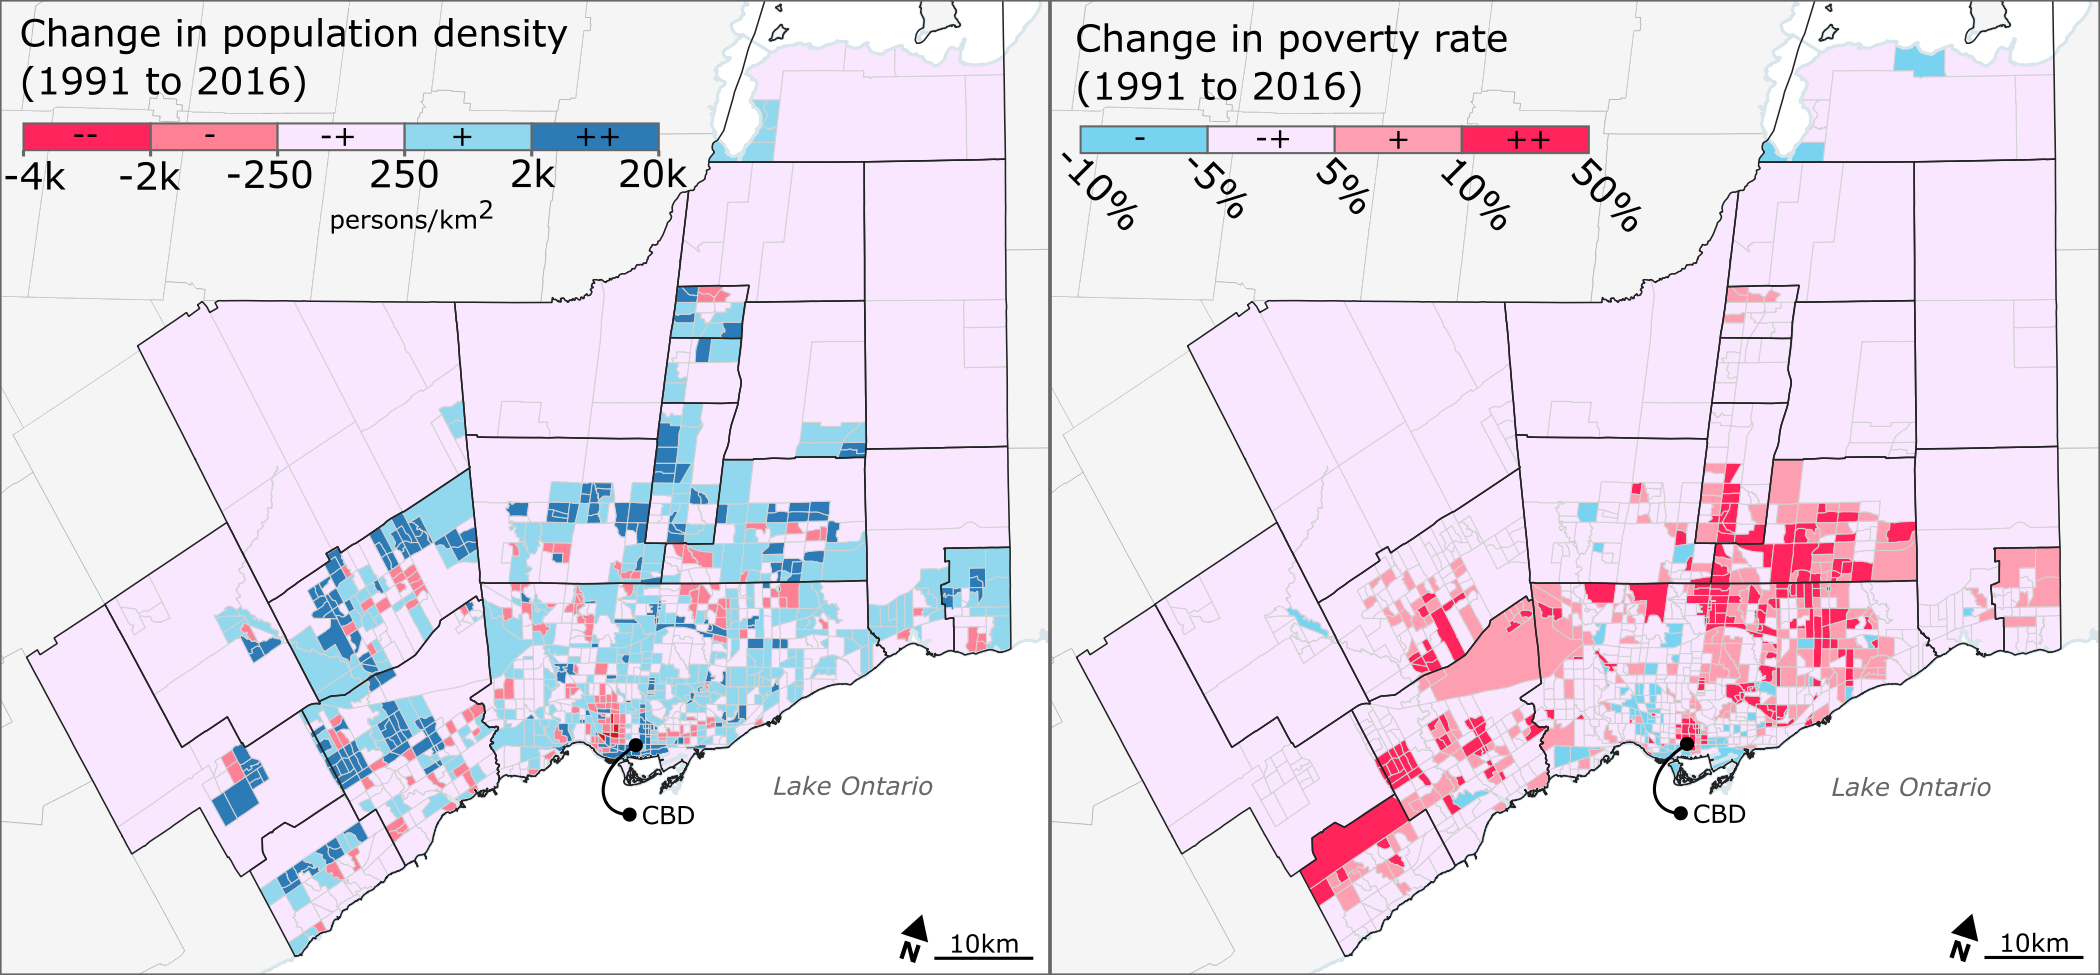
\includegraphics[width=1\linewidth]{figures/study_area_map.png}
	\caption{{Changes in population density and poverty rates in the Toronto CMA (1991 to 2016)}}
	\label{fig:studyareamap}
\end{figure}


While the automobile is the primary mode for most residents in the Toronto CMA (68\% of commuting trips in 2016 were by car), public transit is used by many for daily travel (24\% of commuting trips in 2016) and especially by lower-income residents (32\% of commuting trips in 2016 by low-income workers were by public transit) \cite{government_of_canada_2016_2016}. The Toronto CMA is an agglomeration of several municipalities, each of which operate their own public transit agency, primarily consisting of surface bus routes. The Toronto Transit Commission, the largest municipal transit agency in the region additionally operates surface streetcar routes and a four-line grade-separated rapid transit network. During the time period of our study (1988-2018), the rapid transit network expanded from 3 to 4 lines with a total of 11 new rapid transit stations opening, bringing the total up to 75 stations in the network by 2018. There is also a network of commuter rail and regional bus lines operated by GO Transit, the lone regional transit agency. The 7 commuter rail lines are radially configured, focused on commuting trips to and from the downtown central business district. Several of these lines have undergone expansion from only offering peak-period commuting services to all-day two-way service over the past 25 years. Overall, transit accessibility in the Toronto CMA has been found to be vertically equitable in the sense it serves lower-SES residents more than higher income residents, on average \cite{deboosere_evaluating_2018,allen_sizing_2019}. However, an analysis of neighbourhood socio-economic change relative to transit accessibility and travel behaviour has found that growing poverty in suburban neighbourhoods with low transit accessibility is correlated with increasing adverse travel behaviour outcomes such as decreasing activity participation rates and longer commute times \cite{allen_suburbanization_2021}. 





\section{Data Sources}

The two main sources of data for our study are historical neighbourhood-level transit accessibility measures and individual-level panel data that include variables on residential location and household income. 

Place-based measures of potential accessibility, originally formalized by Hansen \cite{hansen_how_1959}, are commonly used to assess the socio-economic distributions of the benefits derived from transport networks and land-use within a region and over time \cite{manaugh_who_2012,pereira_future_2019}. Place-based measures of transit accessibility for our study were based on the following commonly used potential accessibility formulation \cite{hansen_how_1959,levinson_towards_2020}

\begin{equation}
A_{i,t} = \sum_{j \in J} O_{j,t} f(c_{i,j,t})
\end{equation}
\vspace{2mm}

Where $A_{i,t}$ is the accessibility measure for zone $i$ and year $t$, $j \in J$ are the set of destination zones in a region, $c_{i,j,t}$ is the travel cost from zone $i$ to zone $j$, and $O_{j,t}$ is the number of opportunities in a zone, $j$. For our study, we make use of place-based transit accessibility measures that were computed in a previous study that assessed changes in transit accessibility over time in relation to suburbanization of poverty in Toronto from 1991 to 2016 \cite{allen_suburbanization_2021}. These measures were generated from historical travel survey data and travel demand models. Specifically, data on the location of opportunities, $O_{j,t}$ were from quinquennial (1991, 1996, 2001, 2006, 2011, 2016) regional travel survey that represent 5\% of the region's population \cite{ashby_transportation_2016}, and $c_{i,j,t}$ were travel times based on associated retrospective travel demand models \cite{tmg_gtamodel_2016}. The accessibility measures include consideration for both employment and non-work (e.g. discretionary) activity destinations. See \citeA{allen_suburbanization_2021} for further details on these historical transit accessibility measures. Accessibility measures are provided on a scale ranging from 0 to 100 (the maximum value across all years). For our study, we then additionally use linear interpolation to estimate transit accessibility for intermediary years resulting in having transit accessibility measures, $A_{i,t}$, for each census tract, $i$, and every year, $t$, from 1991 to 2016. (Figure \ref{fig:accessmaps} shows transit accessibility measures for 1991 and 2016). Years 1988, 1989, and 1990 are additionally given the values for 1991, and 2017 and 2018 are given the values from 2016. 

This set of transit accessibility measures are then linked to an individual-level panel dataset, the Longitudinal Administrative Databank (LAD). This data is a 20\% sample of tax filers across Canada on an annual basis from 1988 to 2018 \cite{government_of_canada_longitudinal_2020}. Because of privacy issues, the data are accessed at a secure Research Data Centre operated by Statistics Canada. Included in the data are variables on demographics, household composition, low-income status, sampling weights (used for all subsequent analysis), as well as the census tract and postal code of a person's home address on December 31st of each year. We use this geographical information to link the individual data to accessibility measures based on their year, $t$, and census tract, $i$. Importantly, the data also include a dichotomous indicator of low-income status, specifically the Low-Income Measure (LIM). This is a poverty line created by Statistics Canada, defined as half of the adjusted median household in a region, where adjusted is based on the median household income divided by the square root of household size. This accounts for how as a household increases in size, it's monetary needs increase, but at a decreasing rate \cite{government_of_canada_longitudinal_2020}. For our analysis, we term residents under this threshold as "low-income" and those above as "non-low-income"

\begin{figure}[H]
	\centering
	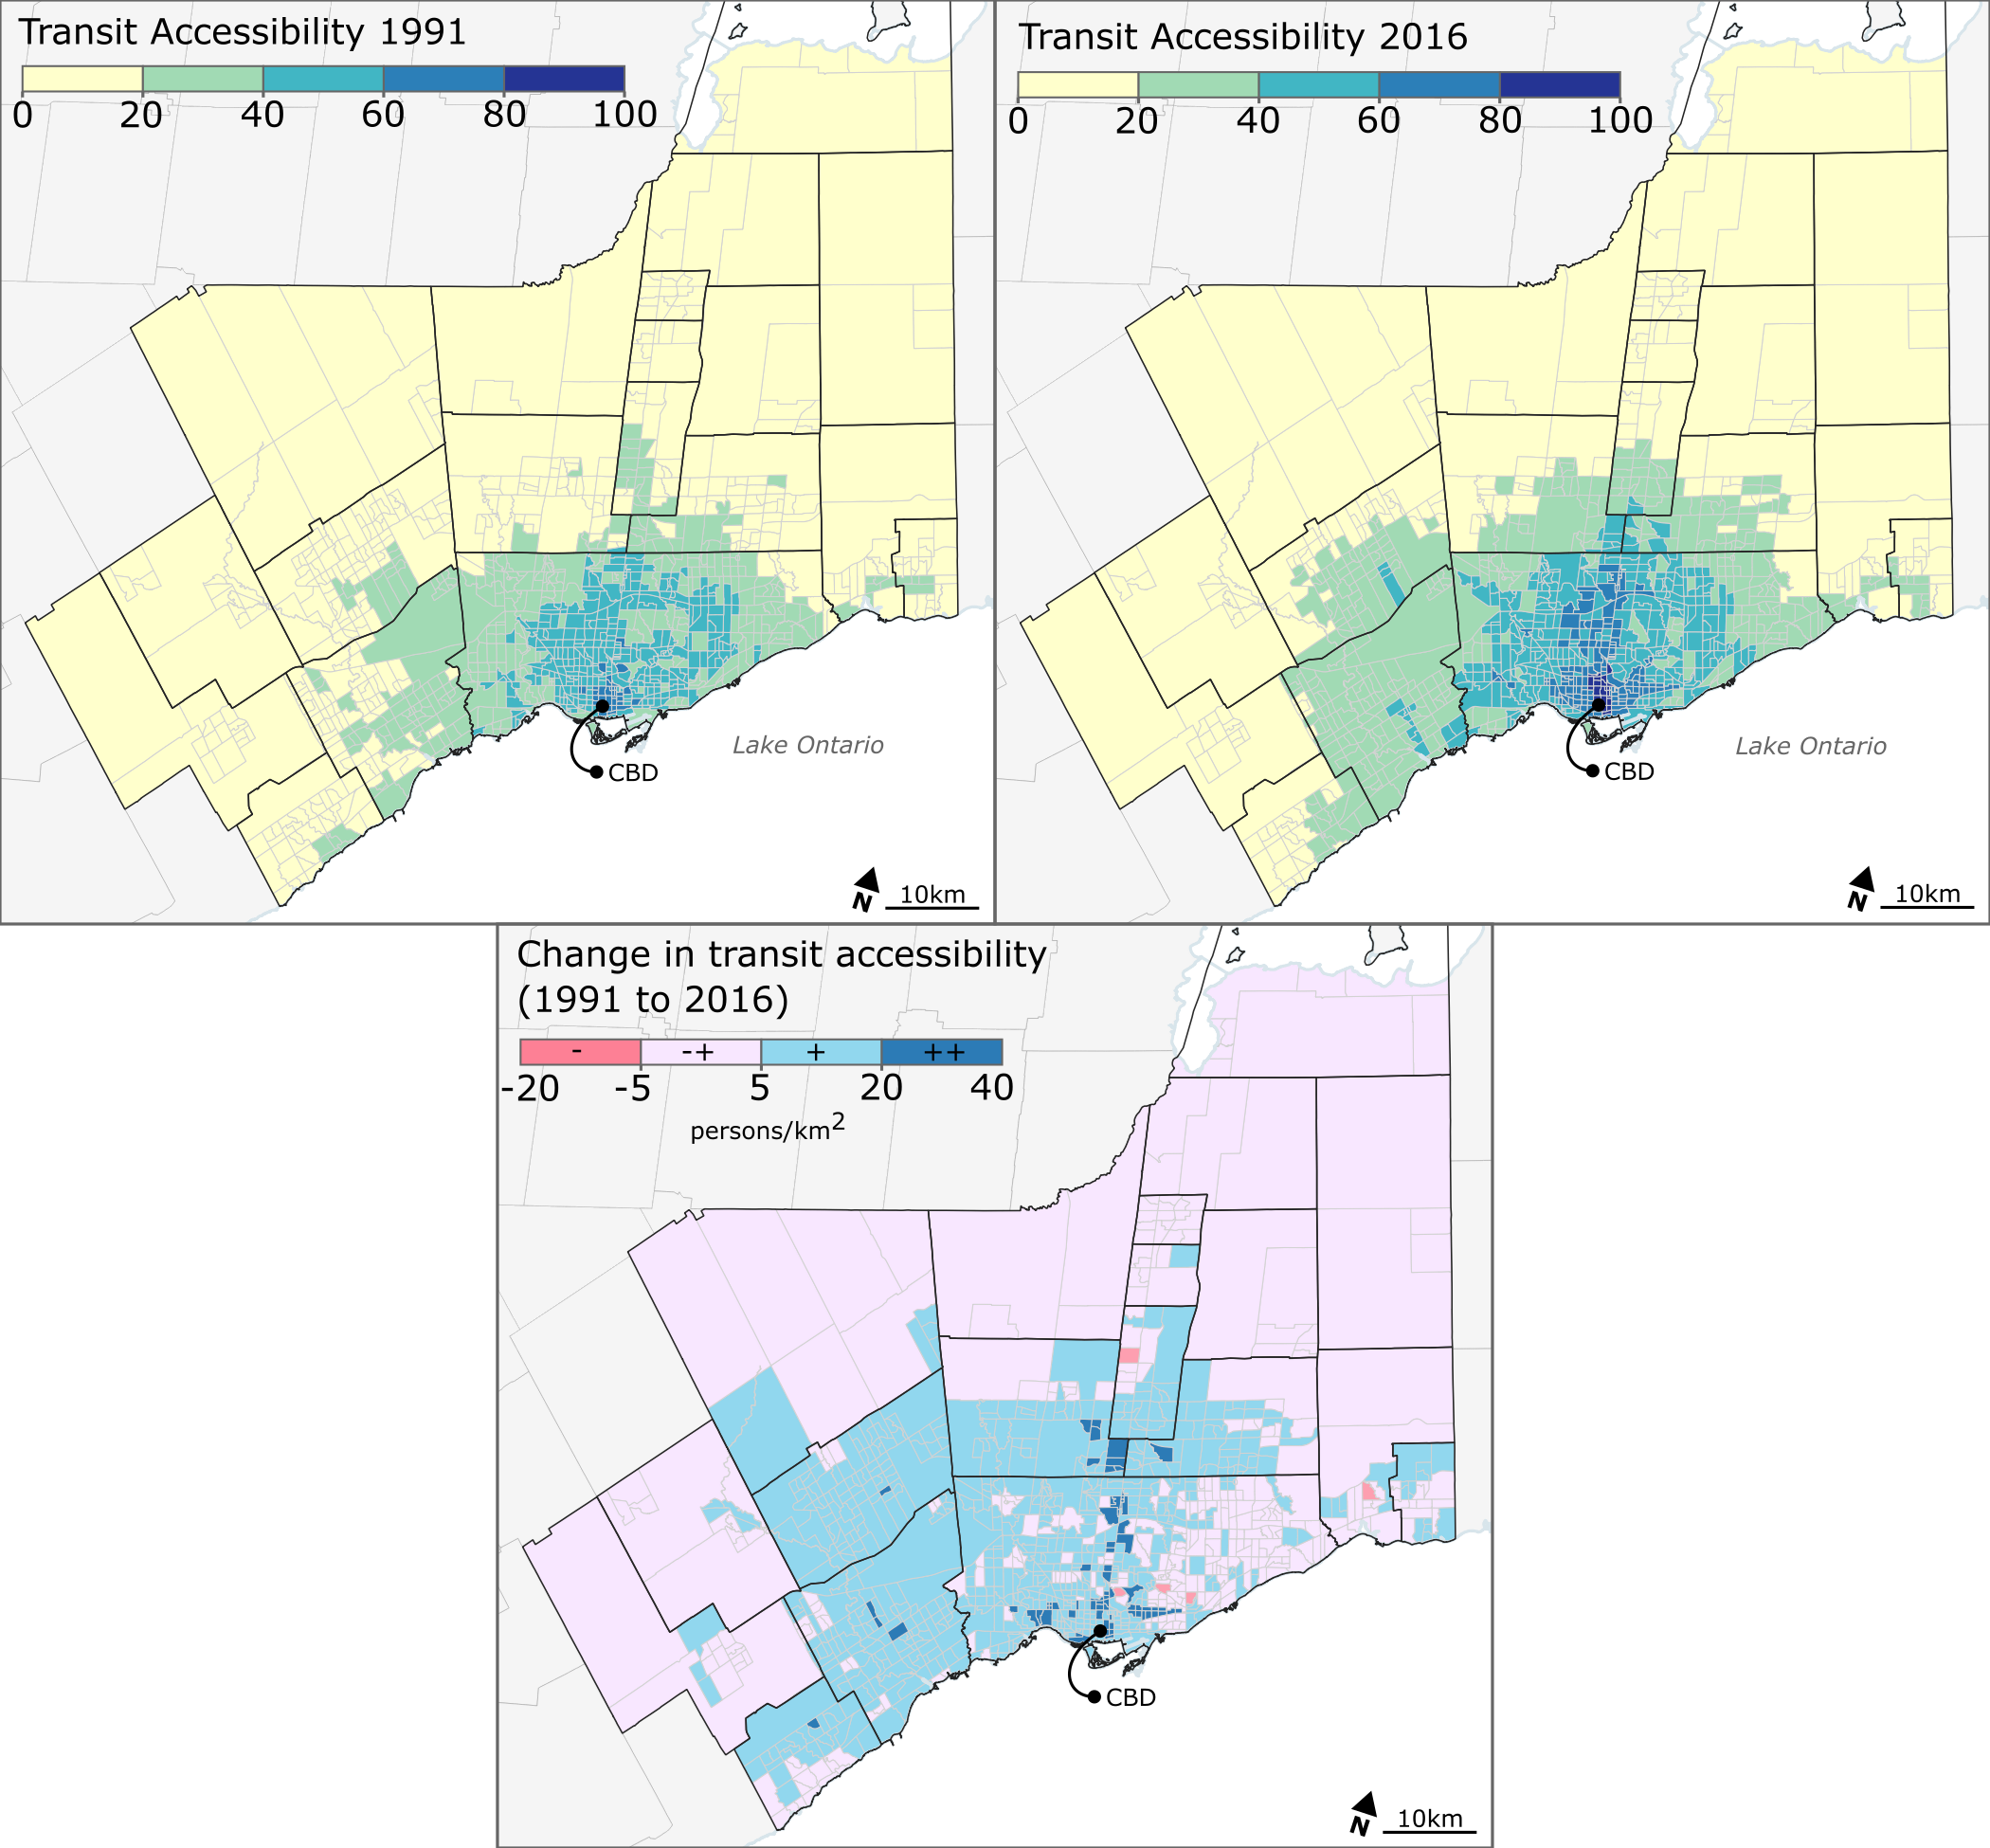
\includegraphics[width=1\linewidth]{figures/acces_mapas.png}
	\caption{{Transit accessibility in Toronto CMA in 1991 and 2016}}
	\label{fig:accessmaps}
\end{figure}



Figure \ref{fig:4plots} displays summary statistics of the Longitudinal Administrative Databank from 1989 to 2018. We find that the poverty rate (\% of the weighted sample in a below LIM household) has increased over time, from approximately 10\% in 1989 to over 20\% 2014, and then declined from 2014 to 2018. The percentage of people who have moved per year has declined over time.  residents move more often than non-low-income households, but this gap has also reduced over time, primarily due to a faster drop in moving rates for low-income residents. Average transit accessibilities have generally increased over time. This is likely due to population growth in areas with good transit accessibility (e.g. downtown) and that most new suburban neighbourhoods have been connected with local bus routes. In some suburban municipalities, there has also been growth in employment which has helped to increase accessibility in nearby neighbourhoods. The data also show that low-income residents, on average, have higher levels of transit accessibility than non-low-income residents throughout this time period.


\begin{figure}[H]
	\centering
	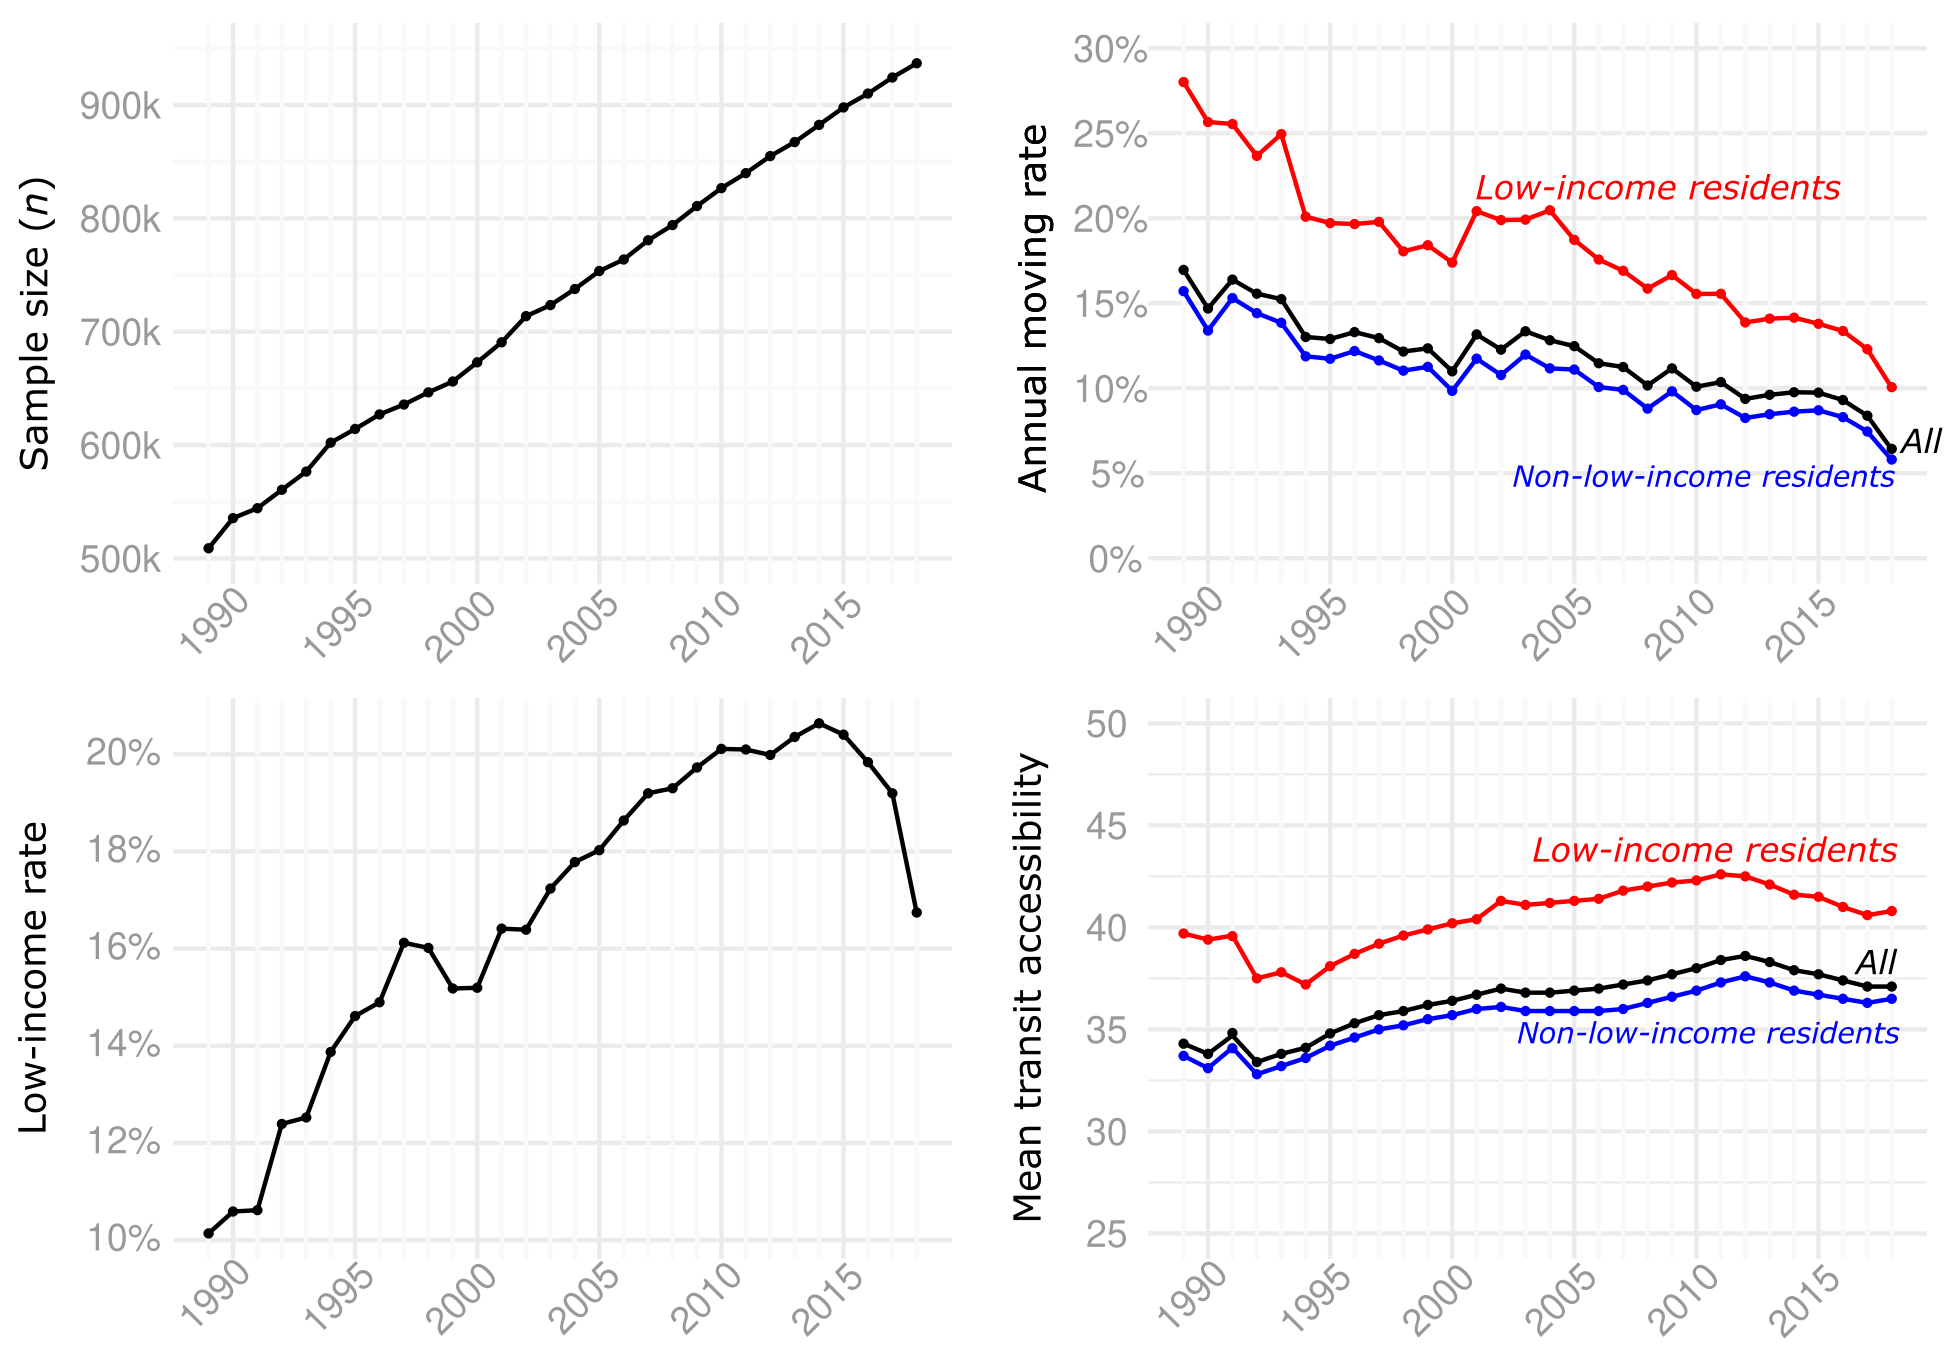
\includegraphics[width=1\linewidth]{figures/4plots.png}
	\caption{{Summary plots of the Longitudinal Administrative Databank and transit accessibility over time}}
	\label{fig:4plots}
\end{figure}




\section{Methods}


From this linked data, we classify whether someone moves if their postal code changes between year $t$ and year $t + 1$. We then compute the absolute difference in transit accessibility, $\Delta A_{k}$, between two years for each mover, $k$, as follows.
\begin{equation}
\Delta A_{k} = A_{i,k,t + 1} - A_{i,k,t}
\end{equation}

A positive value of $\Delta A_{k}$ indicates that a resident has increased their transit accessibility during a move, while a negative value indicates a decrease in transit accessibility. 

For our results, we first create summary statistics and visualizations to show differences in $\Delta A_{k}$ by income status, as well as how this has changed over time. 

We then estimate multivariate regression models to examine if low-income movers are more or less likely to reduce their transit accessibility after controlling for other demographic and household factors that may influence residential mobility to and from different types of neighbourhoods. Because low-income residents have a greater propensity to move (see Figure \ref{fig:4plots}), we use a two-step Heckman selection model to account for how movers are a non-random sample of the overall population. Heckman selection models were initially developed for estimating wages first through labour force participation \cite{heckman_shadow_1974}. In urban transportation research they have been used for analyzing the effects of car ownership and transit accessibility on earnings \cite{smart_disentangling_2020}, analyzing travel distances based on mode choice \cite{kaplan_walking_2016}, and residential moving distances if moved away from new transit infrastructure \cite{chu_impacts_2017}.

The model consists of the following unobserved processes; a selection equation and an outcome equation.
\begin{equation}
m_k^* = \gamma Z_k  + \epsilon_{k,1}
\end{equation}
\begin{equation}
\Delta A_{k}^* = \beta X_{k} + \epsilon_{k,2}
\end{equation}

Where $m_k^*$ and $\Delta A_{k}^*$ are the latent variables for selecting to move and experienced changes in accessibility resulting from a move, respectively, $Z_k$ and $X_{k}$ are vectors of independent variables, $\gamma$ and $\beta$ vectors of coefficients, and  $\epsilon_{k,1}$ and $\epsilon_{k,2}$ are the error terms. In our data, we observe whether people move, and if so, their changes in accessibility. 
\begin{equation}
m_k = 
\begin{cases} 
0 \hspace{1mm} \text{if} \hspace{1mm} m_k^* < 0 \\
1 \hspace{1mm} \text{otherwise}
\end{cases}
\end{equation}
\begin{equation}
\Delta A_{k}  = 
\begin{cases} 
0 \hspace{7mm} \text{if} \hspace{1mm} m_k = 0 \\
\Delta A_{i,k}^* \hspace{1mm} \text{otherwise}
\end{cases}
\end{equation}

The selection equation is modelled as a binomial probit and the outcome as ordinary least squares regression based on the following assumptions.
\begin{equation}
\epsilon_{k,1} \sim N(0,1)
\end{equation}
\begin{equation}
\epsilon_{k,2} \sim N(0,\sigma)
\end{equation}
\begin{equation}
corr(\epsilon_{k,1},\epsilon_{k,2}) = \rho 
\end{equation}

Because of this assumed correlation, the outcome equation includes the inverse Mills ratio based on the linear predictions from the probit selection equation as an additional variable in the outcome equation. The model is estimated via maximum likelihood using the \texttt{sampleSelection} library in $R$. For additional details on model estimation, see Toomet and Henningsen \cite{toomet2008sample}. Models are generated for data from all years pooled into a single dataset, and include a categorical variable for year (this is categorical rather than numeric due to the non-linear temporal relationships shown in the previous plots). Importantly, the independent variables, $X$ and $Z$, include a categorical variable for low-income status. The direction and significance of its coefficient will convey whether low-income residents are more or less likely to reduce their transit accessibility when they move. 


% The expected value for the outcome equation is written as follows:


% \begin{equation}
% E[\Delta A_{i,k} | X_k, m_k = 1] = \beta X_{k} + \rho \sigma \lambda (\gamma Z_k)
% \end{equation}


To round up our study, we categorize transit accessibility into 10 groups (ranked from low to high) using equal intervals (e.g. the lowest is 0-10, the highest is 90-100). We then count how many movers, $N_{u,v,w}$, have moved between different transit accessibility of category, $u$, to category, $v$, by income status, $w$ (i.e. for low- and non-low-income residents) during the study period. Visualizing these flows by accessibility category and income group allows for examining how the more aggregate trends from the previous analyses are possibly due to proportionately low or high out-mobility for each income group or due to residential exclusion at different locations along the spectrum of transit accessibility.




\section{Results}

We begin by visualizing mean changes in accessibility experienced by intra-urban movers. This is shown in Figure \ref{fig:2smooth}. The left figure plots the percent of residents who decrease their levels of transit accessibility when they move. The right figure plots the average change in accessibility, $\Delta A_{k}$, experienced during an intra-urban move. The dashed lines are the means across the entire time period, while the solid lines are local averages fit with a generalized additive model. Overall, residents decrease their transit accessibility, on average, when they move. Looking at the curves, we see fluctuations over time, which likely pertain to core-periphery development trends over time as well. In the early 1990s, residents were more likely to move towards transit, but since 2000, this has hovered around and slightly above the 50\% mark (more residents are moving away from transit). The curves for $\Delta A_{k}$ are consistently less than 0. This is likely partly due to how the newest built suburban neighbourhoods (that thus primarily consist of people moving in, and not out) have some of the lowest transit accessibility in the region. This also indicates that central housing probably has relatively more in-movers from external migration, while peripheral suburban housing has more residents moving in from within the city and thus undergoing a larger reduction in their level of transit accessibility.


\begin{figure}[H]
	\centering
	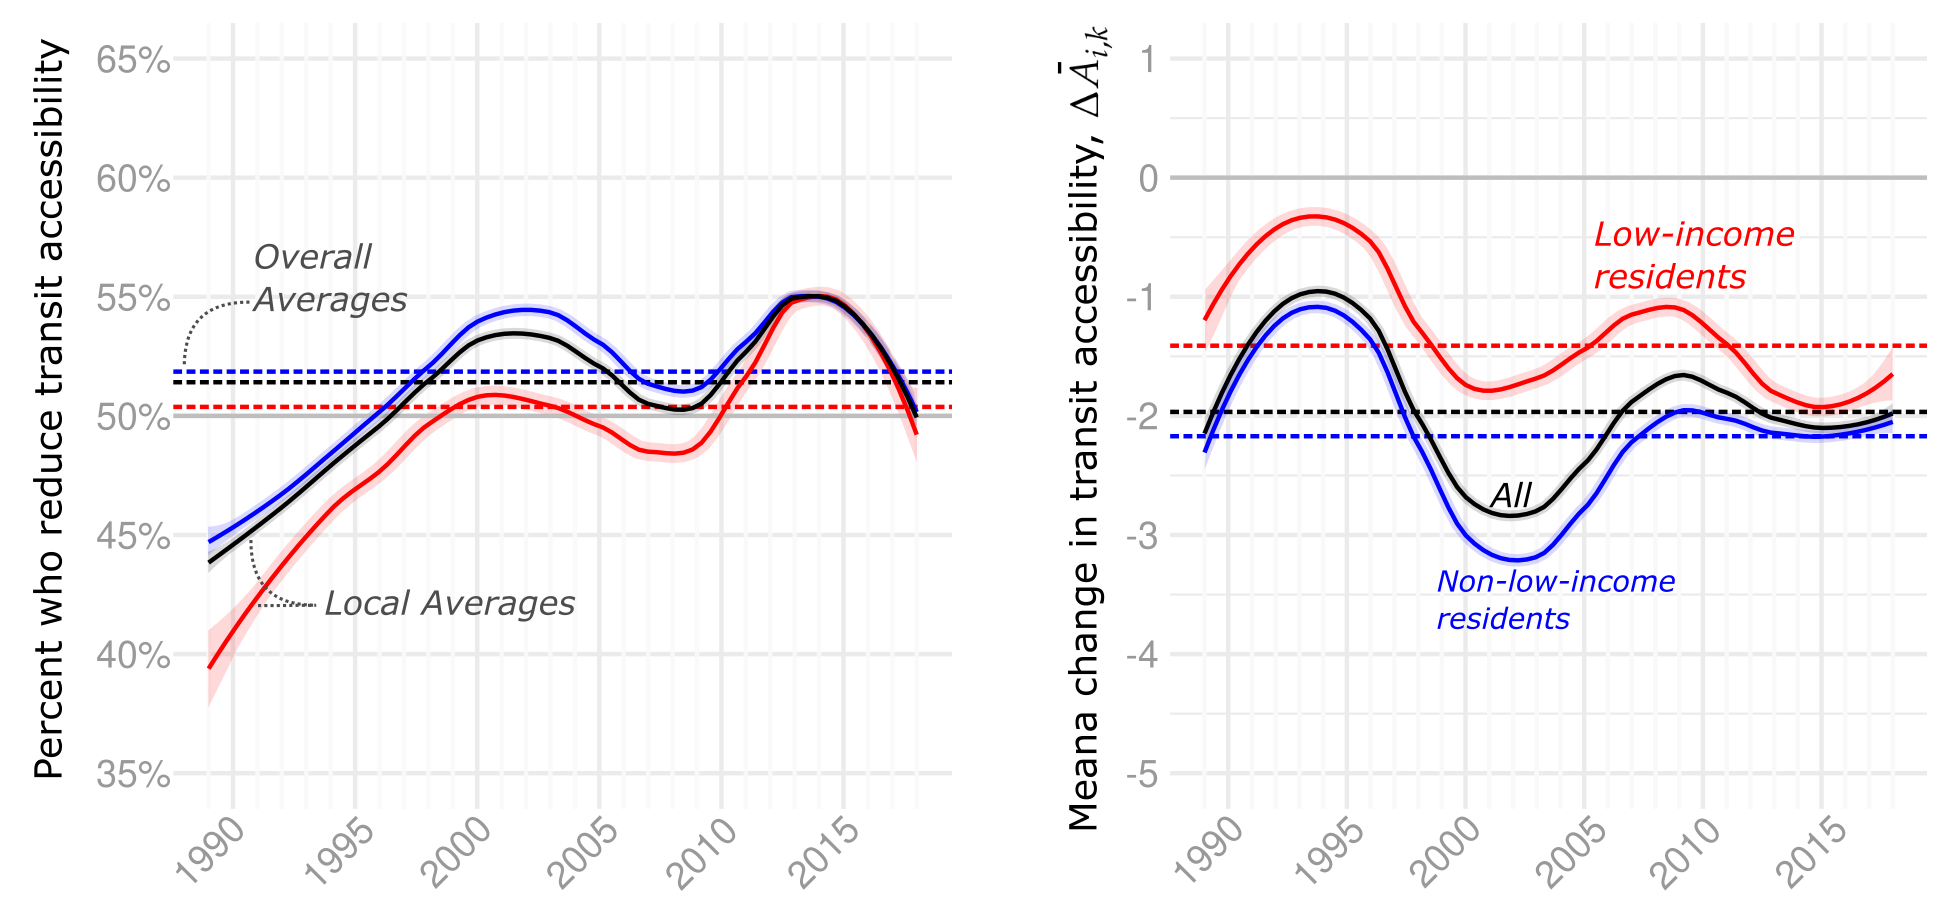
\includegraphics[width=1\linewidth]{figures/2smooth.png}
	\caption{{Changes in transit accessibility for intra-urban movers}}
	\label{fig:2smooth}
\end{figure}

Comparing low-income and non-low-income residents, we find that higher income residents are more likely to decrease their accessibility when moving, and the extent of their reduction is greater as well (the yearly averages are significantly different based on a $t$-test). Therefore, during this study period in Toronto, low-income residents do not decrease their transit accessibility when they move at a greater rate compared to non-low-income residents. However, when looking at the trends over time, we find that the low-income and non-low-income curves converge during the final 10 years of the study period. This is an indication that the effects of gentrification and suburbanization of poverty, at least in terms of residential mobility, are also increasing over time. We find that from 2012 to 2018, low- and non-low-income residents move away from transit at approximately the same rate, but low-income residents still experience less of a reduction in transit accessibility during this time period. This finding could be evidence of residential exclusion in the newest, most peripheral suburbs, as these areas consist of single-family dwellings that are unaffordable for lower-income residents. Also, locations of suburban poverty in Toronto concentrate more within the inner-suburbs, which when viewed regionally, have average levels of transit accessibility. 



These relationships are further examined via the results of regression models displayed in Table \ref{table:models}. Positive coefficients in the selection model ($\gamma > 0$) indicate that the variable has a positive effect on the propensity to move. Confirming the descriptive trends (Figure \ref{fig:4plots}), low-income residents are more likely to move in the past year. Recent immigrants are also more likely to move. Overall this indicates that people living with lower levels of socio-economic status are more likely to experience residential instability and increased propensity to move. Changes in family status, such as having children, children moving in or out, or couples forming or splitting, also increase likelihood of moving, likely due to wanting to change dwellings to suit new household needs.

Positive coefficients in the outcome model ($\beta > 0$) indicate that the variable is more likely to increase the level of transit accessibility during a residential move (each unit increase in $X$ increases transit accessibility by a value of $\beta$ during a move). For low-income status, we find that low-income residents have a change in transit accessibility of 0.84 more than non-low-income residents. Overall, this is not a substantial difference, given that accessibility in this case ranges on a scale of 0 to 100, but still a significant difference. These results also corroborate the descriptive analysis shown in Figure \ref{fig:2smooth}. Aside from income, household factors such as reducing household size, being a lone-parent, being a recent immigrant, and the presence of older children in the household all increase the likelihood of increased transit accessibility when moving. These factors are likely both due to neighbourhood preferences (e.g. for urban neighbourhoods, living near transit) as well as dwelling preferences (e.g. smaller dwelling sizes, which also tend to be more centrally located).



\begin{table}[H]
	
	\renewcommand{\baselinestretch}{1.0} 
	\small
	
	\caption{{Results of Heckman selection models predicting change in transit accessibility for intra-urban movers}}
	\label{table:models}
	
	\begin{adjustwidth}{-1in}{-1in}
		\centering
	\begin{tabular}{lrrrrrrr}
		\hline
		&         &  & \multicolumn{2}{r}{\textbf{Selection Model}}              &                      & \multicolumn{2}{r}{\textbf{Outcome Model}}                \\
		\textbf{Independent Variables$^*$}   &  &  & \multicolumn{1}{c}{$\gamma$} & \multicolumn{1}{c}{$p$} & \multicolumn{1}{c}{} & \multicolumn{1}{c}{$\beta$} & \multicolumn{1}{c}{$p$} \\ \hline
		Intercept                               &         &  & -1.072                   & 0.000                 &                      & -1.289                   & 0.000                 \\
		Income Status in year $t$                   &         &  &                          &                       &                      &                          &                       \\
		\hspace{2mm} Non-low-Income (ref)                         & 82.8\%  &  &                          &                       &                      &                          &                       \\
		\hspace{2mm} Low-Income                                & 17.2\%  &  & 0.186                    & 0.000                 &                      & 0.843                    & 0.000                 \\
		Immigrated between $t - 1$ and $t$             &         &  &                          &                       &                      &                          &                       \\
		\hspace{2mm} No (ref)                                  & 98.6\%  &  &                          &                       &                      &                          &                       \\
		\hspace{2mm} Yes                                       & 1.4\%   &  & 0.284                    & 0.000                 &                      & 0.279                    & 0.000                 \\
		Sex                                       &         &  &                          &                       &                      &                          &                       \\
		\hspace{2mm} Female (ref)                              & 52.3\%  &  &                          &                       &                      &                          &                       \\
		\hspace{2mm} Male                                      & 47.7\%  &  & 0.008                    & 0.000                 &                      & 0.033                    & 0.004                 \\
		Age in year $t$                             &         &  &                          &                       &                      &                          &                       \\
		\hspace{2mm} 18 to 25 (ref)                            & 13.0\%  &  &                          &                       &                      &                          &                       \\
		\hspace{2mm} 26 to 35                                  & 20.3\%  &  & 0.060                    & 0.000                 &                      & -1.180                   & 0.000                 \\
		\hspace{2mm} 36 to 45                                  & 21.3\%  &  & -0.165                   & 0.000                 &                      & -0.974                   & 0.000                 \\
		\hspace{2mm} 46 to 55                                  & 18.0\%  &  & -0.349                   & 0.000                 &                      & -0.520                   & 0.000                 \\
		\hspace{2mm} 56 to 65                                  & 12.7\%  &  & -0.535                   & 0.000                 &                      & -0.312                   & 0.000                 \\
		\hspace{2mm} 66 to 75                                  & 8.6\%   &  & -0.660                   & 0.000                 &                      & -0.097                   & 0.286                 \\
		\hspace{2mm} 76 and up                                 & 6.2\%   &  & -0.587                   & 0.000                 &                      & -0.895                   & 0.000                 \\
		Family type in year $t$                     &         &  &                          &                       &                      &                          &                       \\
		\hspace{2mm} Couple with children                      & 46.9\%  &  &                          &                       &                      &                          &                       \\
		\hspace{2mm} Couple without children           & 24.7\%  &  & 0.171                    & 0.000                 &                      & -0.361                   & 0.000                 \\
		\hspace{2mm} Lone parent           & 8.0\%   &  & 0.198                    & 0.000                 &                      & 1.613                    & 0.000                 \\
		\hspace{2mm} Single/roommates              & 20.3\%  &  & 0.351                    & 0.000                 &                      & 1.792                    & 0.000                 \\
		Number of children in year $t$              &         &  &                          &                       &                      &                          &                       \\
		\hspace{2mm} Children aged 0 to 4                      & $\mu = $ 0.15    &  & 0.069                    & 0.000                 &                      & -0.607                   & 0.000                 \\
		\hspace{2mm} Children aged 5 to 9                      & $\mu = $ 0.16    &  & -0.020                   & 0.000                 &                      & -0.227                   & 0.000                 \\
		\hspace{2mm} Children aged 10 to 14                    & $\mu = $ 0.17    &  & -0.014                   & 0.000                 &                      & -0.058                   & 0.000                 \\
		\hspace{2mm} Children aged 15 to 18                    & $\mu = $ 0.16    &  & -0.116                   & 0.000                 &                      & 0.011                    & 0.597                 \\
		\hspace{2mm} Children aged 19 and up                   & $\mu = $ 0.38    &  & -0.261                   & 0.000                 &                      & 0.316                    & 0.000                 \\
		Change in rel. status between $t$ and $t + 1$ &         &  &                          &                       &                      &                          &                       \\
		\hspace{2mm} No change (ref)                           & 91.2\%  &  &                          &                       &                      &                          &                       \\
		\hspace{2mm} Couple split up                           & 3.0\%   &  & 0.827                    & 0.000                 &                      & 3.823                    & 0.000                 \\
		\hspace{2mm} Became a couple                           & 5.8\%   &  & 0.051                    & 0.000                 &                      & -2.013                   & 0.000                 \\
		New baby in the hhld between $t$ and $t + 1$            &         &  &                          &                       &                      &                          &                       \\
		\hspace{2mm} No (ref)                                  & 97.4\%  &  &                          &                       &                      &                          &                       \\
		\hspace{2mm} Yes                                       & 2.6\%   &  & 0.094                    & 0.000                 &                      & -1.101                   & 0.000                 \\
		Change in children moving in/out from $t$ to $t + 1$        &         &  &                          &                       &                      &                          &                       \\
		\hspace{2mm} No change (ref)                   & 88.7\%  &  &                          &                       &                      &                          &                       \\
		\hspace{2mm} More children moved in                         & 4.5\%   &  & 0.398                    & 0.000                 &                      & -0.894                   & 0.000                 \\
		\hspace{2mm} More children moved out                        & 6.9\%   &  & 0.837                    & 0.000                 &                      & 2.448                    & 0.000                 \\ \hline
		&         &  &                          &                       &                      &                          &                       \\
		\textbf{Model parameters}                  &   $n$   &    & Statistic & $p$                          &                                            &                          &                       \\ \hline
		$\sigma$                                     &         &  & 21.506                   & 0.000                 &                      &                          &                       \\
		$\rho$                                       &         &  & -0.043                   & 0.000                 &                      &                          &                       \\
		$n$ overall                             &           21,821,785  &  &              &                       &                      &                          &                       \\
		$n$ movers                               &            2,512,020 &  &               &                       &                      &                          &       \\ \hline          
		\multicolumn{8}{p{12.2cm}}{\small{$^*$ Categorical variables for year are displayed in Table \ref{table:models_2}}}\\
		
	\end{tabular}
	\end{adjustwidth}
	
\end{table}




\begin{table}[H]
	\renewcommand{\baselinestretch}{1.0} 
	\small
	\centering
	\caption{{Coefficients for year for the Heckman selection models presented in Table \ref{table:models}}}
	\label{table:models_2}
	\begin{tabular}{lrrrrrrr}
		\hline
		&         &  & \multicolumn{2}{r}{\textbf{Selection Model}}              &                      & \multicolumn{2}{r}{\textbf{Outcome Model}}                \\
		\textbf{Year}   &  &  & \multicolumn{1}{c}{$\gamma$} & \multicolumn{1}{c}{$p$} & \multicolumn{1}{c}{} & \multicolumn{1}{c}{$\beta$} & \multicolumn{1}{c}{$p$} \\ \hline
		
		1988 (ref) & 2.3\% &  &                   &                 &  &                  &                \\
		1989       & 2.4\% &  & -0.152            & 0.000           &  & 1.259            & 0.000          \\
		1990       & 2.5\% &  & -0.058            & 0.000           &  & 0.029            & 0.450          \\
		1991       & 2.6\% &  & -0.081            & 0.000           &  & 1.099            & 0.000          \\
		1992       & 2.6\% &  & -0.078            & 0.000           &  & 1.506            & 0.000          \\
		1993       & 2.8\% &  & -0.153            & 0.000           &  & 1.808            & 0.000          \\
		1994       & 2.8\% &  & -0.146            & 0.000           &  & 1.500            & 0.000          \\
		1995       & 2.9\% &  & -0.124            & 0.000           &  & 1.177            & 0.000          \\
		1996       & 2.9\% &  & -0.130            & 0.000           &  & 0.727            & 0.000          \\
		1997       & 3.0\% &  & -0.167            & 0.000           &  & 0.483            & 0.000          \\
		1998       & 3.0\% &  & -0.142            & 0.000           &  & -0.109           & 0.017          \\
		1999       & 3.1\% &  & -0.211            & 0.000           &  & -0.167           & 0.001          \\
		2000       & 3.2\% &  & -0.102            & 0.000           &  & -0.434           & 0.000          \\
		2001       & 3.3\% &  & -0.093            & 0.000           &  & -0.498           & 0.000          \\
		2002       & 3.3\% &  & -0.087            & 0.000           &  & -0.313           & 0.000          \\
		2003       & 3.4\% &  & -0.094            & 0.000           &  & -0.257           & 0.000          \\
		2004       & 3.4\% &  & -0.116            & 0.000           &  & 0.108            & 0.015          \\
		2005       & 3.5\% &  & -0.163            & 0.000           &  & 0.152            & 0.002          \\
		2006       & 3.6\% &  & -0.169            & 0.000           &  & 0.527            & 0.000          \\
		2007       & 3.6\% &  & -0.230            & 0.000           &  & 0.758            & 0.000          \\
		2008       & 3.7\% &  & -0.167            & 0.000           &  & 0.649            & 0.000          \\
		2009       & 3.8\% &  & -0.228            & 0.000           &  & 1.033            & 0.000          \\
		2010       & 3.8\% &  & -0.208            & 0.000           &  & 0.549            & 0.000          \\
		2011       & 3.9\% &  & -0.274            & 0.000           &  & 0.057            & 0.321          \\
		2012       & 4.0\% &  & -0.250            & 0.000           &  & 0.173            & 0.002          \\
		2013       & 4.0\% &  & -0.239            & 0.000           &  & 0.386            & 0.000          \\
		2014       & 4.1\% &  & -0.246            & 0.000           &  & 0.355            & 0.000          \\
		2015       & 4.2\% &  & -0.266            & 0.000           &  & 0.256            & 0.000          \\
		2016       & 4.2\% &  & -0.331            & 0.000           &  & 0.227            & 0.000          \\
		2017       & 4.3\% &  & -0.612            & 0.000           &  & 0.799            & 0.000 
		\\ \hline
	\end{tabular}
\end{table}






In the results in Figure \ref{fig:2smooth} and Table \ref{table:models}, we find that low-income residents are less likely than high income residents to decrease transit accessibility when moving. To provide further nuance into these findings, we first plot the percent of residents by income group moving out of different intervals of transit accessibility during the study period (Figure \ref{fig:res_acc_inc} left). This shows that in the highest accessibility areas, non-low-income residents are more likely to move out compared to non-low-income residents the lowest accessibility neighbourhoods. The trend is different for low-income residents, who move out less often in the highest and lowest accessibility areas, but move more out of neighbourhoods in the middle of the accessibility spectrum (these neighbourhoods approximately correspond to the inner-suburbs, and the greater percents in inner suburbs may be due to the high concentrations of recent immigrants in some of these neighbourhoods). Overall, these results indicate that despite trends of gentrification in areas of high transit accessibility, low-income residents are not moving out at a disproportionate rate. This finding is similar to those in the United States \cite{freeman_displacement_2005,delmelle_new_2020}. 

Figure \ref{fig:res_acc_inc} (right) shows the percent of in-movers into each interval of transit accessibility by income group. This plot indicates that the areas of the lowest accessibility, i.e. rural areas, exurbs, and peripheral suburbs are more exclusive for non-low-income residents - rather than middle or high accessibility neighbourhoods. Overall, non-low-income residents having a greater propensity to move out of high-accessibility neighbourhoods and into the lowest-accessibility neighbourhoods is a key reason why they decrease their transit accessibility when moving more than low-income residents.


\begin{figure}[H]
	\centering
	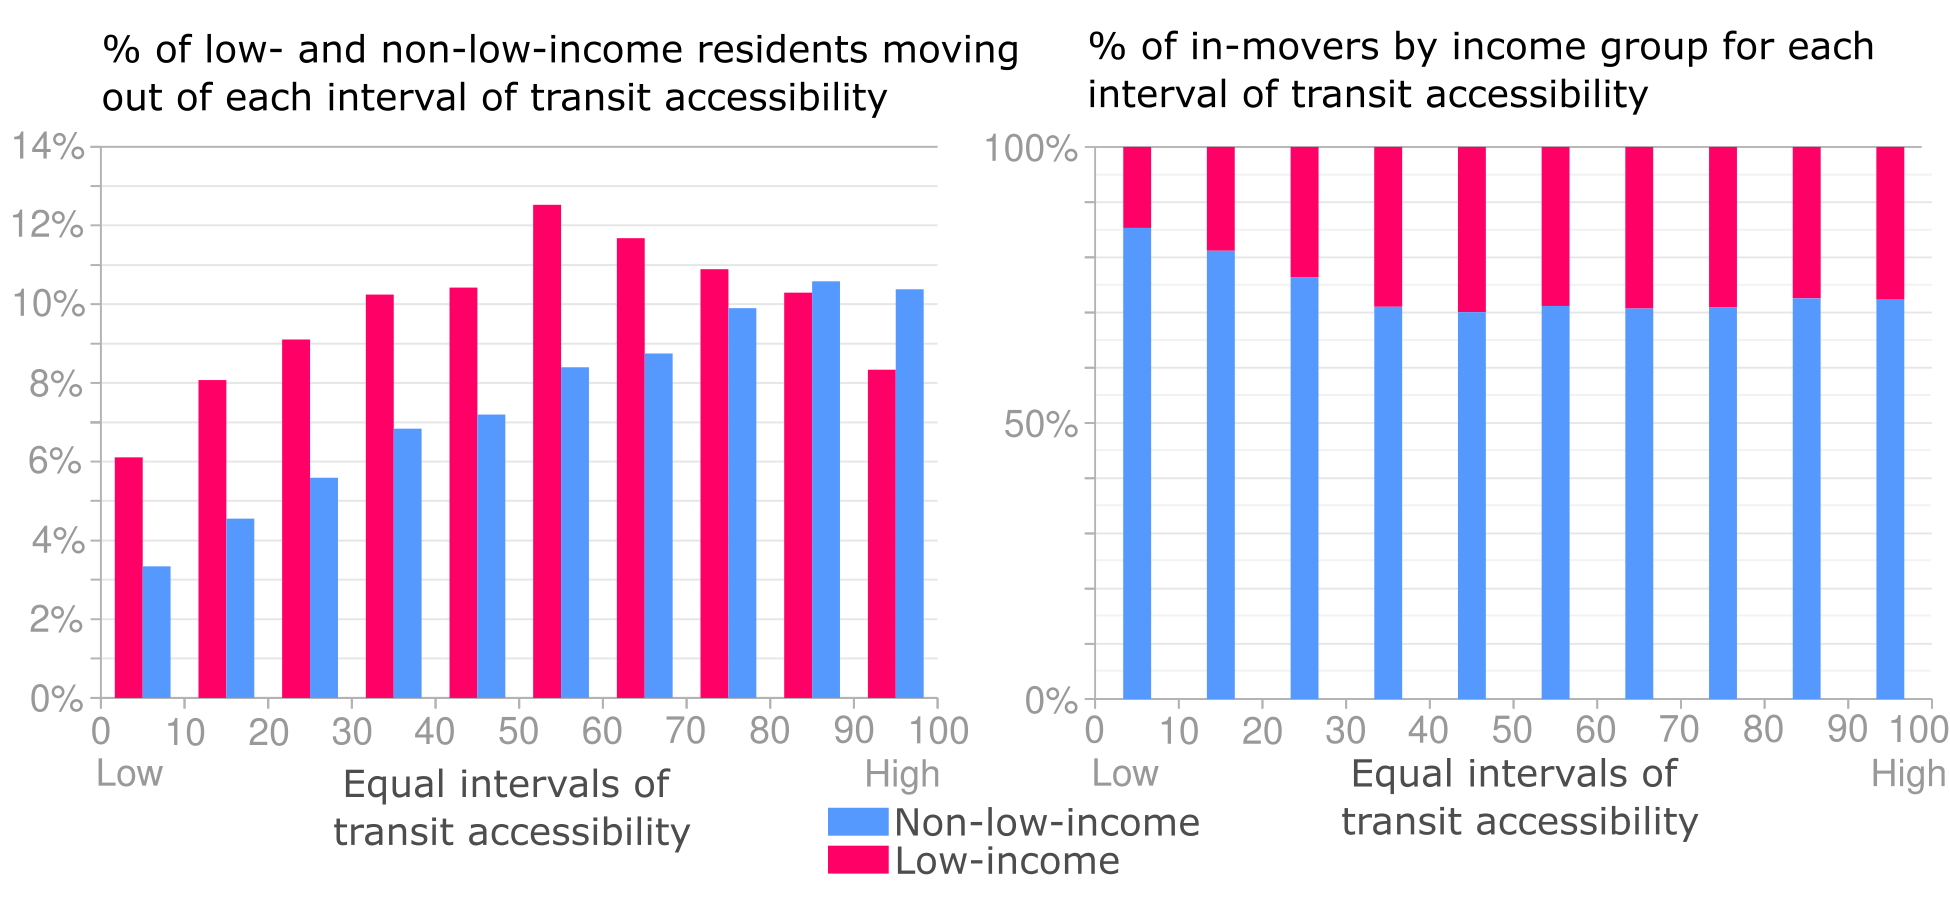
\includegraphics[width=1\linewidth]{figures/res_acc_inc_bars.png}
	\caption{{In and out movers by income and equal intervals of transit accessibility}}
	\label{fig:res_acc_inc}
\end{figure}





\section{Conclusions}

In our analysis, we find that low-income residents, on average, decrease their transit accessibility when they move. This has important social inclusion implications since many low-income residents are reliant on public transit for travelling to daily activities \cite{allen_planning_2020,barri_can_2021}, including finding employment \cite{fransen_relationship_2019,bastiaanssen_does_2021}. Moving away from relied upon public transit could thus decrease capabilities for activity participation, and in some cases, increase risks of transport-related social exclusion \cite{lucas_transport_2012,allen_planning_2020}.

However, we also find that low-income residents do not decrease their transit accessibility when moving at a greater rate than non-low-income residents. This is despite ample neighbourhood-level research describing inner-city gentrification occurring in Toronto over the past several decades \cite{hulchanski_three_2010,walks_gentrification_2021}. In fact, we find that non-low-income residents living in central areas are more likely to move out of these neighbourhoods than compared to low-income residents, and on average experience greater reductions in their levels of transit accessibility when they move. This difference in findings is likely because the unit of analysis of our study were individuals rather than neighbourhoods, meaning that gentrification observed at a neighbourhood level is likely partly due to upward income mobility of residents who stay in these neighbourhoods or affluent residents moving in from outside the study region (either national or international immigrants). As well, we also find that much of the outward residential mobility by non-low-income households noted in 20th century urban theory \cite{burgess_growth_1925,alonso_location_1964} has continued to persist in Toronto. In particular, the outer suburbs and exurbs of Toronto are predominately exclusive to non-low-income residents compared to other areas. 

Even though low-income residents are not disproportionately moving away from transit relative to non-low-income residents, gentrification and increasing costs of housing are still likely leading to changing spatial patterns of low-income neighbourhoods in the region. In Toronto, the most affordable housing is located in the inner-suburbs as mid-20th century apartment towers \cite{skaburskis_filtering_2014,august_gentrification_2018}. The formation of low-income neighbourhoods in these inner-suburban neighbourhoods, but without evidence of substantial displacement and residential exclusion in central neighbourhoods, indicates that these observed increases in suburbanization of poverty in Toronto is more likely due to immigrants with lower incomes settling in the suburbs or residents becoming and remaining poor in-place within the suburbs.

Overall, it would be difficult to generalize the findings from our analysis to other regions. However, the methods we presented could be replicated elsewhere. This would certainly be doable in other Canadian contexts as the panel dataset we used is available Canada-wide \cite{government_of_canada_longitudinal_2020}, but it would require additional sources for historical transit accessibility measures elsewhere (we only had this data available for Toronto). Conducting a comparative analysis across multiple cities would be an important direction for future work to assess whether there are consistencies or differences in findings regarding whether low-income residents are unequally moving away from transit. Similarly, future research could examine how results might vary using different definitions of accessibility and thresholds for low-income status, possibly as part of a sensitivity analysis. For example, our historical travel survey data were limited in that we could only look at access to all jobs within a region, rather than low-income jobs. Moreover, while the objective of our study was to examine changes across an entire region, another important direction for future work would be to map at a more localized scale whether there are neighbourhoods that have undergone high rates of out-mobility of low-income residents, and specifically if out-movers are decreasing their transit accessibility when moving, even if these trends are not prevalent at an aggregate regional level. This could provide more direct evidence into the locations within a region that are potentially experiencing residential displacement away from relied-upon public transit service.